\documentclass[]{article}
\usepackage[a4paper,left=2.54cm, right=2.54cm, top=2.54cm, bottom=2.54cm, footskip=0.5cm]{geometry}		% footskip = Abstand zwischen 
\usepackage{amsmath} %Never write a paper without using amsmath for its many new commands
\usepackage{amssymb} %Some extra symbols
\usepackage{appendix}
\usepackage{graphicx}
\usepackage{eurosym}
\usepackage{dcolumn} % for tables
\usepackage[sort&compress]{natbib}
\usepackage[pdftex]{hyperref}

\graphicspath{{./Figures/}}


%opening
\title{Public support for global vaccine sharing in the COVID-19 pandemic: Intrinsic, material, and strategic drivers\footnote{Research for this contribution is part of the Cluster of Excellence "Contestations of the Liberal Script" (EXC 2055, Project-ID: 390715649), funded by the Deutsche Forschungsgemeinschaft (DFG, German Research Foundation) under Germany´s Excellence Strategy.}}
\author{Ferdinand Geissler, Humboldt-Universität zu Berlin \\
	Felix Hartmann, Humboldt-Universität zu Berlin \\ 
	Macartan Humphreys, WZB Berlin Social Science Center/Columbia University \\
	Heike Klüver, Humboldt-Universität zu Berlin \\
	Johannes Giesecke, Humboldt-Universität zu Berlin
}

\begin{document}

\maketitle

\begin{abstract}
As of early November 2021 an estimated 40\% of the global population is fully vaccinated for Covid-19 but the global distribution of vaccines is extremely unequal, with over 80\% vaccinated in the top 10 countries and below 1\% in the bottom 10. Given that governments need to secure public support for investments in global vaccine sharing, it is important to understand the levels and drivers of public support for international vaccine solidarity. Using a  factorial experiment administered to more than 10,000 online survey respondents in Germany, we show that global inequities are out of line with German public opinion. Respondents are supportive of substantive funding amounts, on the order of the most generous contributions provided to date, though still below amounts that are likely needed for a successful global campaign. Public preferences appear largely to be driven by intrinsic concern for the welfare of global populations though are in part explained by material considerations---particularly risks of continued health threats from a failure to vaccinate globally. Strategic considerations are of more limited importance in shaping public opinion; in particular we see no evidence for free riding on contributions by other states. Finally, drawing on an additional survey experiment, we show that there is scope to use information campaigns to augment public support further.   
\end{abstract}


\newpage


\section{Introduction}

Vaccination is the key to overcome the COVID-19 pandemic. Multiple vaccines have been developed in record time and more than 7 billion doses billion doses have been administered globally to date.  %While only 0.3\% of people in low-income countries are fully vaccinated, as much as 43.7\% of the population in high-income countries are fully vaccinated.\footnote{Source: https://github.com/favstats/vacccprogress} 
As of early November 2021 an estimated 40\% of the global population is fully vaccinated. However, the global distribution of the COVID vaccines is extremely unequal. While over 80\% of citizens are vaccinated in the ten countries leading in the COVID vaccination campaign, less than 1\% of the population is vaccinated in the ten least performing countries. Strikingly, per capita GDP alone explains as much as  60\% of the variation in vaccination rates; COVID mortality about 6\%.\footnote{Numbers calculated from data from Our World in Data; calculations available in replication materials.}  

Besides the evident inequities, and the economic and health threats to poorer countries \citep{egger2021falling}, the unequal provision of vaccines has important consequences for wealthier countries. The risks from low global provision include economic and health threats  arising from continued interruptions of global supply chains, and the preservation of reservoirs that facilitate disease mutation. One study estimates global costs at \$9 trillion \citet{agarwal2021proposal}. It has been estimated that  approximately 70\% of the worldwide population must be fully vaccinated to end the COVID-19 pandemic \citep{Randolph2020}. The delta variant has pushed the threshold for global herd immunity to  80\% and potentially approaching 90\% \citep{barker2021rethinking}.  Thus, vaccine inequity is not only a humanitarian disaster, it is one that has direct material consequence for wealthier countries. 

Researchers at the International Monetary Fund (IMF) estimate the costs of global vaccination at \$50 billion \citep{agarwal2021proposal}. Other estimates put costs closer to \texteuro 80 billion.  Though there is no clear determination of what a fair share is, as a benchmark, if the richest 25\% of countries provided \texteuro 70 per citizen this would sum to 80 billion Euros and imply contributions of about \texteuro 6 billion for Germany and \texteuro 23 billion for the United States. Using the Fair Share calculation, based on OECD guidelines, Germany's share of OECD donor shares would be \$5bn (8\% of \$63bn).\footnote{For details see \citet{care2021}.}  

However, a fair distribution of COVID-19 vaccines is not only a matter of providing money, but vaccines will continue to be scarce for some time. Despite the importance of globally distributing COVID-19 vaccines to stop the pandemic, a number of Western countries have launched campaigns for a third booster vaccination in the wake of the fourth wave of the pandemic which currently hits countries with full force \citep{Mahase2021}. Poorer countries will struggle obtaining  sufficient vaccines for their citizens in the foreseeable future. On 4 August 2021, WHO director Tedros Adhanom Ghebreyesus therefore called for a moratorium halting COVID-19 vaccine boosters in favor of unvaccinated.\footnote{Source: \href{https://www.reuters.com/business/healthcare-pharmaceuticals/who-calls-moratorium-covid-19-vaccine-booster-doses-until-september-end-2021-08-04/}{Reuters}} 


Given that governments need to secure public support either for making large monetary contributions or for sharing vaccines with poorer countries, it is important to understand the levels and drivers of public support for global vaccine sharing and to identify ways through which governments can increase solidarity with other countries in need. Previous research has focused on ethical questions of global vaccine distribution \citep{Emanuel2020,Jecker2021} or on  mapping the international distribution of COVID-19 vaccines \citep[e.g.][]{Massinga2021,Katz2021}. However, little is known about public opinion on global vaccine sharing. In this study we focus on three motivations: \textit{intrinsic} motivations, \textit{material} motivations, and \textit{strategic} motivations. By intrinsic motivations we refer to the preferences for sharing that derive from concern for the wellbeing of global populations. By material incentives we refer to the economic and health benefits to German citizens that might arise from a global response. To assess strategic motivations we draw on related literatures on contributions to global public goods. In particular, past work on European solidarity during the Eurozone crisis \citep{Bechtel2017,Kuhn2018,Kuhn2020,Stoeckel2018} and preferences for international climate agreements \citep{Bechtel2019},  highlights how popular preferences by both the specific costs and benefits for the donor country and the design of multilateral agreements. Building on this work we examine both the role of (stipulated) direct costs to Germany and the structure of international cooperation.  We also assess the extent to which public support can be increased through information campaigns appealing to the self-interest of citizens. 


% Vaccination is the key to overcome the COVID-19 pandemic. A number of vaccines have been developed in record time and 6 billion doses have been administered globally to date. However, the global distribution of the vaccines is extremely unequal. While only 0.3\% of people in low-income countries are fully vaccinated, as much as 43.7\% of the population in high-income countries are fully vaccinated.\footnote{Source: https://github.com/favstats/vacccprogress} 


%Of course cash is not the only way to meet needs. In addition, countries can help provide vaccines directly, or provide support by for instance extending intellectual property rights and know-how. Direct donation of vaccines is limited by supply however and sets up a starker distributional challenge. Indeed allocations are currently being administered to provide third vaccinations---booster shots---in wealthy countries, before first vaccinations are given in poorer ones \citep{Mahase2021}.  On 4 August 2021, WHO director Tedros Adhanom Ghebreyesus therefore called for a moratorium halting COVID-19 vaccine boosters in favor of unvaccinated citizens in poorer countries.\footnote{Source: https://www.reuters.com/business/healthcare-pharmaceuticals/who-calls-moratorium-covid-19-vaccine-booster-doses-until-september-end-2021-08-04/}. Hence,  vaccines against COVID-19 will continue to be scarce  and poorer countries will struggle obtaining  sufficient vaccines for their citizens in the foreseeable future.


Our results show that  German citizens are supportive of generous contributions to the global distribution of vaccines against COVID-19. Median popular support is somewhat below estimated contributions needed to fund global vaccine redistribution; though average amounts exceed this. Popular preferences for global vaccine solidarity  appear to primarily stem from humanitarian concerns and are only in part explained by material and strategic considerations. While there is a preference for multilateral efforts, public support for large contributions to global vaccine distribution does not depend  on the behavior of other countries. We furthermore show that information campaigns can increase public support for international vaccine solidarity. 

Overall the stark inequalities in global vaccine distribution are not in line with public opinion. Vaccine nationalism, though evident in policy, is a minority position. The results of our study have implications for the current public debate on global vaccine distribution, but also for international solidarity and international cooperation more generally. On the one hand, the COVID-19 vaccination is a highly salient issue for all citizens worldwide and thus provides a unique opportunity to study popular preferences for international solidarity. On the other hand, since herd immunity is a global public good as the pandemic can only be overcome if all countries worldwide are immunized, our findings can furthermore inform the literature on preferences for international cooperation. 



%%%%%%%%%%%%%%%%%%%%%%%%%%%%%%%%%%%%%%%%%%%%%
%%%%%%%%%%%%%%%%%%%%%%%%%%%%%%%%%%%%%%%%%%%%%


\section{Design}
\label{sec:design}


Our analysis draws on data generated from a factorial survey experiment implemented as part of a five-wave panel study on vaccine attitudes that was fielded in Germany in 2021. We employ data primarily from wave 4 of the project which was administered to 10,525 respondents between 8 and 22 September 2021 (for details, see the Supporting Information (SI)). Our population of interest is all German citizens between 18 and 75. We rely on a representative sample which was drawn with the help of the online-access panel provider \hspace{0pt}Respondi\hspace{0pt}\hspace{0pt}. All analyses were specified in a preregistered analysis plan made available at the Center for Open Science (https://osf.io/69mpy) and the study obtained IRB approval at Humboldt-Universität zu Berlin (HU-KSBF-EK$\_$2021$\_$0010 and HU-KSBF-EK$\_$2021$\_$0019).


%During the field time of the wave 2 survey, only 7.7 (29 April) to 9.7 (10 May) per cent of the population was fully vaccinated while 19 (29 April) to 24 (10 May) per cent had received the first dose.\footnote{Source: https://ourworldindata.org/covid-vaccinations} At the same time, 77 per cent of the respondents indicated that they either were already vaccinated (33 per cent), that they definitely want to get vaccinated against COVID-19 (44 per cent) or that they were undecided (11 per cent). Hence, at the time when we conducted the experimental study, COVID vaccines were an extremely scarce good as public demand greatly exceeded the supply with vaccines. 

In the experiment, participants were twice  asked to consider hypothetical situations which randomly varied along four dimensions (health benefits, economic benefits, no of countries participating, contribution of other countries). In each case, respondents were asked to indicate how   much Germany should contribute to global vaccine sharing, both in \texteuro  and in vaccine doses.

More specifically, two dimensions focused on the benefits of global vaccine sharing for Germany in terms of public health and in terms of economic growth. One asked participants to imagine that ``The risk of new mutations of the coronavirus increases considerably in Germany if there are no vaccinations in poorer countries"; a second asked participants to imagine that ``The German economy shrinks by around 5\% if there are no vaccinations in poorer countries." For each of these a control condition was provided in which there were no costs to Germany if there are no vaccinations in poorer countries.

The other two dimensions focused on the nature of multilateral agreements, asking participants to imagine settings in which 0, 20 or 40 countries took part, contributing collectively \texteuro 0, \texteuro 20, or \texteuro 40 billion. In all there are five types of agreement considered (because 0 participants implies 0 contributions and vice versa). In all this gives rise to a $2\times2\times5$ factorial design. 


%
% Before implementation of the experiment, we collected a number of covariates to examine to what extent international vaccine solidarity is moderated by individual attitudes and attributes. We included trust in government and local health system \citep{Mesch2015}, economic hardship and education \citep{Bertoncello2020}, minority group status and maternal age \citep{Danis2010}, risk
%perception \citep{Brewer2007} and health status \citep{Guay2019}. Additionally, we collect data on political attitudes, attitudes towards migrants, and attitudes towards COVID-19 as well as indicators that identify groups who are eligible for the vaccine.\footnote{Please see the questionnaire in the Supplementary Materials for more details.}
% 

%%%%%%%%%%%%%%%%%%%%%%%%%%%%%%%%%%%%%%%%%%%%%
%%%%%%%%%%%%%%%%%%%%%%%%%%%%%%%%%%%%%%%%%%%%%

\section{Results}
\label{sec:results}


\subsection{Levels of support for vaccine solidarity}

Figure \ref{fig:hist1} graphs raw data patterns to show the share of Germans supporting contributions of \texteuro $X$ or less (top panel) or $X$ donations of vaccine doses (bottom panel) or less. We indicate, separately, preferred contributions when there are large economic and health costs of the status quo for Germany (versus none) and situations in which there is a major international deal (versus none).

We see that median contributions are around \texteuro 2 billion and 100 million doses,  an amount closely in line with actual current German commitments.%(source). 
There is considerable heterogeneity, however, with about one third support commitments around \texteuro 5 bn or more. A small share---around 1 in 8, support much larger contributions. Given the skewed nature of the distributions, the average amount proposed is much larger --- around  \texteuro 8 billion for cash, but the mean number of doses proposed is lower at around 80 million. 

\begin{figure}[hbt!]
	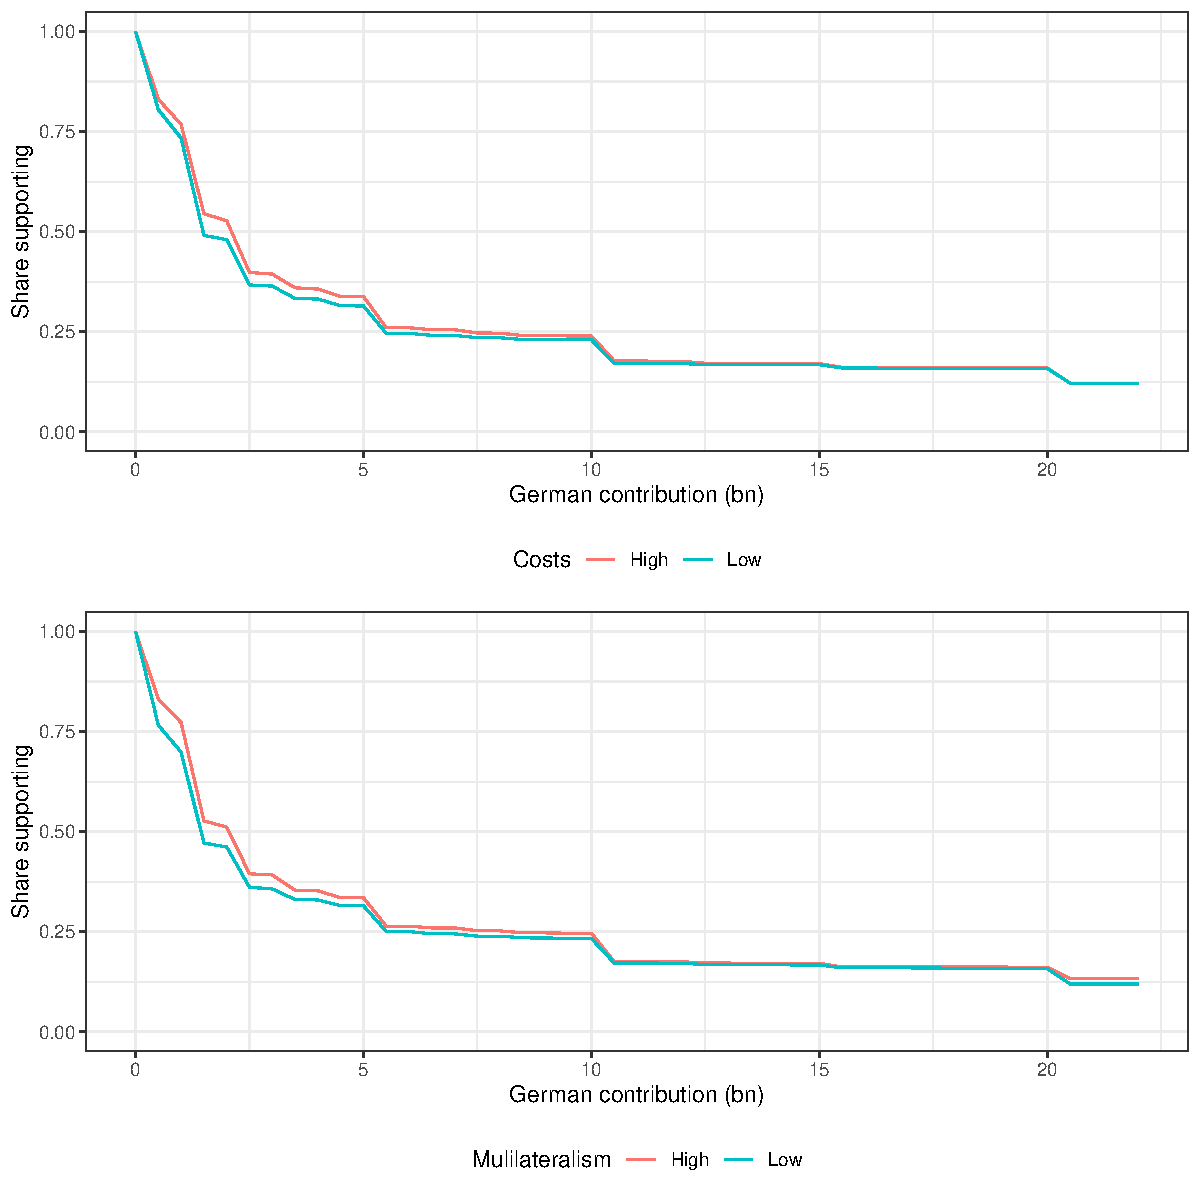
\includegraphics[width=\linewidth]{"../2_output/cumulative.pdf"}
	\caption{Distribution of support for contributions of different sizes}
	\label{fig:hist1}
	%\floatnote{This is a note for this figure.}
\end{figure}

In supplementary material we document variation in these levels of support across subgroups. Using preregistered analyses we show first, that support varies substantially as a function of political party support--- with the greatest support among Green and SPD voters, and weakest support among AfD voters. Second we show variation as a  function of migration background, with substantially greater support for higher levels of contribution among respondents with a migration background. We note nevertheless that despite his variation, support is high in all groups. To wit, a majority of AfD supporters, the group least likely to support international vaccine solidarity, still support contributions of \texteuro 1bn  or more.  

\subsection{Treatment effects}

In Figure \ref{fig:hist1}  we can also see that both sets of conditions increase the size of contribution supported by survey participants. These differences are generally statistically significant (see below) but as seen from the raw data, the effects are quantitatively small. 


Figure \ref{fig:main1} shows the marginal effects of all conditions on optimal cash donations and doses. This represents the same underlying patterns as seen in Figure \ref{fig:hist1} though the focus here is on average effects. Overall we see that both health risks and trading importance are statistically distinguishable from zero, but, as seen already, the magnitude of effects is not large. 

Strikingly the amounts offered are positively responsive to amounts given by others, but unresponsive to the number of others giving. This is the opposite to what one might expect from accounts that focus on free-riding between states, and suggests, rather, a willingness to support initiatives regardless of average contributions by others. 

\begin{figure}[hbt!]
	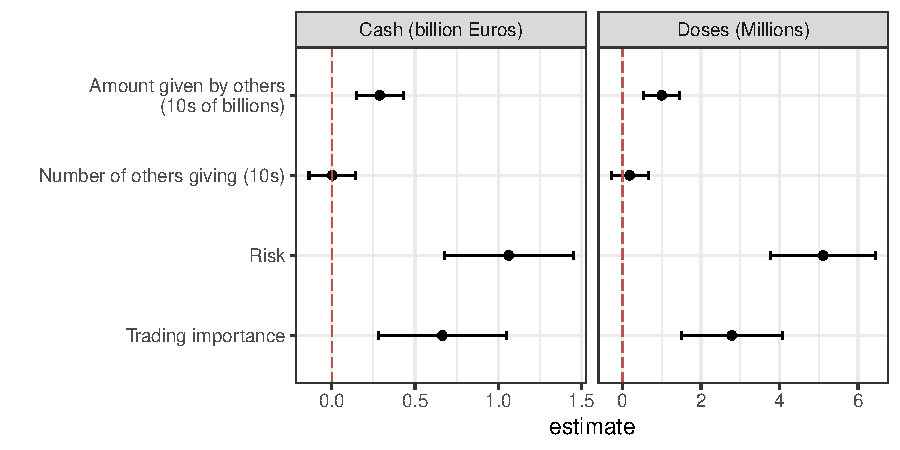
\includegraphics[width=\linewidth]{"../2_output/E1_main.pdf"}
	\caption{Marginal effects of conditions}
	\label{fig:main1}
	%\floatnote{This is a note for this figure.}
\end{figure}

Our heterogeneity analysis (in appendix) suggest that these treatment effects are quite similar for respondents that support different parties or that have different migration backgrounds. The groups 

\subsection{Structural analysis}

Preregistered structural estimation lets us shed more light on the intrinsic, material, and strategic motivations of respondents.

For this analysis we we assume that individuals evaluate own country ($y_i$) and other country ($(y_j)$) contributions according to the objective function:

$$u =  (\alpha + \beta\times \text{economic risk} + \delta \times \text{health risk})  \times \log \left(\sum_{-i}y_j + y_i \right) - \gamma\times(y_i - \kappa\overline{y})^2 - y_i^2 $$

where $\overline{y}$ is the average contribution of other states, and $\sum_{-i}{j_j}$ is the total contributions by others.\footnote{We note that this expression differs from the expression in our pre-analysis plan in not subscripting parameters by respondent.} 

The function assumes diminishing marginal returns to total contributions, convex costs of own contributions, substitutibility of own and other contributions for global benefits, and a possible desire to benchmark contributions against the contributions of others.  Letting $y_i^*$ denote optimal own contributions given economic and health risks and the contributions of others, we assume that players report $y_i^* + \epsilon_i$ where $\epsilon_i \sim N(0,\sigma^2)$. 

We estimate parameters ($\alpha$, $\beta$, $\delta$, $\gamma$, $\kappa$, $\sigma$) using maximum likelihood implemented via bbmle::mle2 in R. The estimated structural parameters are given in Table \ref{tab:structural}.

\begin{table}[!h]

\caption{\label{tab:structural}Structural parameter estimates}
\centering
\begin{tabular}[t]{crrrrrr}
\toprule
parameter & estimate & std.error & statistic & p.value & conf.low & conf.high\\
\midrule
$\alpha$ & 240.62 & 2.01 & 119.73 & 0.00 & 236.68 & 244.56\\
$\beta$ & -10.32 & 12.71 & -0.81 & 0.42 & -35.23 & 14.59\\
$\delta$ & 37.79 & 12.45 & 3.04 & 0.00 & 13.40 & 62.19\\
$\gamma$ & 0.61 & 0.07 & 9.22 & 0.00 & 0.48 & 0.75\\
$\kappa$ & 5.22 & 0.40 & 13.06 & 0.00 & 4.44 & 6.00\\
\addlinespace
$\sigma$ & 15.98 & 0.08 & 205.18 & 0.00 & 15.83 & 16.14\\
\bottomrule
\end{tabular}
\end{table}



We see here strong evidence for marginal gains from contributions independent of economic and health risks ($\alpha$), these marginal gains are increased ($\delta$) when there are substantial health risks (by about 16\%) but are not much affected by economic risks ($\beta$). Respondents place weight on alignment with others ($\gamma$) but the results on $\kappa$ suggest that they target contributions that are significantly higher (five times higher) than the average amount given by others. Note that average contributions by others was not provided directly to respondents, though it can be calculated from the numbers given and the amounts given. 

Overall these results support the conclusions that German respondents see intrinsic benefits from global contributions, that these are augmented, but do not depend on externalities---health externalities in particular---and that Germans, insofar as they benchmark contributions to those of other nations, value contributing at significantly higher rates.



\section{Discussion}

Overall our findings suggest high levels of support for contributions to address global vaccine inequity that stem from intrinsic, material, and, less forcefully, strategic rationales. Two pieces of additional analysis provide support for these conclusions. One provides direct evidence for humanitarian motivations and a second provides direct behavioral evidence for responsiveness to global risks.  



First, we interpret the high rates of giving in the control conditions---when there are no health or economic benefits stipulated---as evidence of non-strategic humanitarian concerns. To measure humanitarian motivations directly we included in the survey (wave 2 and wave 4) a question asking respondents to indicate how  the German government should prioritize to ensure vaccination for an older Indian woman as compared to a younger German woman. The comparison directly pits nationalist concerns against humanitarian concerns. Importantly also, we expect, any strategic considerations that enter in the decision to prioritize an Indian woman should apply \textit{a fortiori} to the prioritization of a German woman. Strikingly, we find that 57\% of the respondents place the priority of the older Indian woman as high or higher than the German woman, and 38\% even place it strictly higher. 



Second, we interpret the results on health and economic costs as indicative of strategic considerations. These considerations are in principle manipulable. In  a second experiment implemented in wave 2, participants were randomly assigned to a \emph{treatment group} that is exposed to a video explaining the benefits of global vaccine sharing and a \emph{control group} which did not see the video. The video emphasizes in particular the risk of more mutations forming if vaccines are not made available in developing countries. Subsequently, respondents were asked whether they support the international distribution of vaccines (attitudinal outcome) and were offered the opportunity to donate money to UNICEF which was put in charge for global vaccine sharing (behavioural outcome). More specifically, respondents earned 75 so-called ``Mingle Points'' cents for their participation in the survey which corresponds to 0.75 Euros. We offered them  50 additional Mingle Points and gave them the following choice. They could either keep the 50 Mingle Points for themselves  or donate all or part of them to UNICEF for the worldwide distribution of Corona vaccines. For every point they donated, we donated 1.5 Euro Mingle points to UNICEF (see table \ref{table:mingle} in the Supplementary Materials). 



We find that respondents in the treatment group that were exposed to the video are significantly more likely to show solidarity both with regard to the attitudinal and the behavioural outcome. More specifically, the reported willingness to personally support international distribution of vaccines is 0.069 units higher than in the control group. In a similar vein, the actual donations that respondents made to UNICEF were on average significantly higher in the treatment than in the control group (details in Figure \ref{fig:video} in SM). 



Before concluding we discuss a set of plausible threats to validity.  The first relates to a set of critique in \citep{diamond1994contingent} that highlights difficulties that respondents have in providing numeric valuations of public goods. Focusing on contingent valuation surveys in Economics, \citep{diamond1994contingent}  highlight risks that respondents may not have well defined valuations of public goods, may not be in a position to take relevant budget constraints into account (which can lead to what is sometimes called an embedding effect), and provide answers that cannot easily be assessed against revealed preferences. Although our experiment bears similarities with contingency valuation surveys our aim here is not to assess individual willingness to pay for global vaccinations but rather to assess what policies respondents would like to see public officials follow. Their report of these preferences to us, which in turn get communicated publicly, albeit in aggregated form, bears a direct relation to the policy quantities of interest which is absent for contingency valuation surveys; by the same token, embedding effects may indeed be real in the formulation of policy priorities. But that does not imply a bias in measurement but rather a threat of inconsistencies in policy demands.  

Although the aim of our survey is different to those of scholars assessing the valuation of public goods, we still recognize that survey responses may not accurately predict the policy preferences that would advocate in a policy context when the benefits and costs of different strategies are debated by political actors, and responses may be sensitive to question wording, for instance, or the information we supplied to contextualize costs.  Fully addressing these questions would require implementing a field analogue of our study, perhaps involving discussions between politicians and citizens \citep{wuttke2021making}.
    

\section{Conclusions}


Our findings have clear implications for the current debate on international vaccine solidarity in the COVID pandemic. With regard to the instruments of achieving a fair allocation of vaccines globally, the evidence presented in Figures \ref{fig:hist1} and \ref{fig:main1} shows that patterns of support for monetary and dose donations are similar. However, the value of median preferred dosage donations (around 100 million doses) is likely substantively smaller than the median preferred cash donations. This is in part an artifact of the fact that dosage donations by Germany are capped by vaccine holdings; nevertheless it highlights the fact that framing sharing in terms of vaccines rather than cash, by suggesting a zero sum nature of the problem, may yield weaker support for sharing. There are, however, many other avenues to address vaccine inequality including strategies that target production in developing countries, through financing, extending intellectual property rights, and sharing know-how.



While efforts to share vaccines globally have been a failure to date, the evidence we provide furthermore suggests that this is not due to lack of public support for the proposition. Average proposals exceed current contributions by the German government and also exceed fair share calculations of what the German government ought to be providing. \textit{Median} proposals are somewhat less than the fair share benchmark, but nevertheless large. Evidence from our experiment with ancillary data suggest that strategic considerations matter, but are not paramount in explaining public preferences. Rather humanitarian rationales loom large. In all, these results suggest that policy-makers who take up the mantel of addressing the challenge of achieving global vaccination will have the moral support of the public behind them.



\newpage
%% Use \bibliography{...} if using BibTeX
\bibliography{solidarity}
\bibliographystyle{apsr}

%TC:subst \printbibliography \bibliography
%TC:macro \field [0,1]
%TC:macro \name [0,0,0,1]
%TC:macro \list [0,0,1]
%% Use \printbibliography if using BibLaTeX
% \printbibliography

\clearpage
%%%%%%%%%%%%%%%%%%%%%%%%%%%%%%%%%%%%%%%%%%%%%%%%%%%%%%% 
\setcounter{page}{1}

\begin{center}
	\appendix{\textbf{\Large{Supplementary Materials}}}
\end{center}



%%%%%%%%%%%%%%%%%%%%%%%%%%%%%%%%%%%%%%%
\tableofcontents


\clearpage

\section{Experiment Design}

We implement a \(2\times2\times5\) factorial design.

We lead with introductory text:

\begin{quote}
	The following is about vaccination progress in Germany and the rest of
	the world.
\end{quote}

\begin{quote}
	The vaccination campaign against the coronavirus in Germany is now well
	advanced and anyone who wanted to be vaccinated could do so. The
	benefits of a third booster vaccination are currently being discussed.
	In contrast, many other, poorer countries are still at the very
	beginning with vaccinations and almost no one there has received a
	single vaccination yet.
\end{quote}

\begin{quote}
	A total of around 11 billion vaccine doses are needed to vaccinate all
	people around the world who are ready to vaccinate. Although the
	production of vaccines is in full swing, there is currently not enough
	vaccine available to carry out the first and second vaccinations in the
	poorer countries and the third vaccination in the richer countries at
	the same time
\end{quote}

\begin{quote}
	Variations are then as follows:
\end{quote}

\textbf{Z1: Trading importance}

\begin{itemize}
	\item
	0 Control: It has no negative impact on the German economy if there
	are no vaccinations in poorer countries.
	\item
	1 Treatment: The German economy shrinks by around 5\% if there are no
	vaccinations in poorer countries.
\end{itemize}

\textbf{Z2: Risk}

\begin{itemize}
	\item
	0 Control: The risk of new mutations of the coronavirus does not
	increase noticeably in Germany if there are no vaccinations in poorer
	countries.
	\item
	1 Treatment: The risk of new mutations of the coronavirus increases
	considerably in Germany if there are no vaccinations in poorer
	countries.
\end{itemize}

\textbf{Z3: Deal}

\begin{itemize}
	\item
	0 Control: There is no international deal on the global distribution
	of vaccines to poorer countries.
	\item
	1 Treatment: There is an international deal on the global distribution
	of vaccines to poorer countries. 20 other countries are involved in
	the agreement, which together contribute a total of 20 billion euros.
	\item
	2 Treatment: There is an international deal on the global distribution
	of vaccines to poorer countries. 40 other countries are involved in
	the agreement, which together contribute a total of 20 billion euros.
	\item
	3 Treatment: There is an international deal on the global distribution
	of vaccines to poorer countries. 20 other countries are involved in
	the agreement, which together contribute a total of 40 billion euros.
	\item
	4 There is an international deal on the global distribution of
	vaccines to poorer countries. 40 other countries are involved in the
	agreement, which together contribute a total of 40 billion euros.
\end{itemize}

Note that \(Z3\) can itself be interpreted as a \(2*2+1\) sub design
that can be coded into:

\begin{itemize}
	\item
	Z4: 0, 20, 40 other countries
	\item
	Z5: 0, 20, 40 billion provided by others
\end{itemize}

\hypertarget{assignment-1}{%
	\subsection{Assignment}\label{assignment-1}}

Each subject sees two conditions, producing a total of
\(20 \times 19 = 380\) versions, assigned independently.

\hypertarget{outcomes-1}{%
	\subsection{Outcomes}\label{outcomes-1}}

Subjects are asked about amounts of vaccines that Germany should share
and financial contributions Germany should make in each condition.

Outcome 1:

\begin{quote}
	The total costs to meet global vaccination needs amount to around 70
	billion euros. A contribution from Germany of one billion euros to this
	fund would cost the population in Germany the equivalent of around 12
	euros per person.
	
	For each of the two scenarios, please indicate how many euros Germany
	should contribute to this fund for global vaccination. (Options range
	from 0 to 70 billion; Millions can be specified, separated by commas
	(e.g.~0.1 billion for 100 million))
\end{quote}

\begin{itemize}
	\item
	Vignette 1 ..billion Euro
	\item
	Vignette 2 ..billion Euro
\end{itemize}

Outcome 2:

\begin{quote}
	Germany will still have around 200 million vaccine doses available by
	the end of the year. If Germany wanted to offer all of its citizens a
	third vaccination, Germany would have to reserve around 70 million of
	these vaccine doses.
\end{quote}

\begin{quote}
	For each of the two scenarios, please indicate what proportion of these
	200 million vaccine doses Germany should contribute to the global
	distribution of vaccine doses to poorer countries. (Options range from 0
	to 200m)
\end{quote}

\begin{itemize}
	\item
	Vignette 1 ..million doses
	\item
	Vignette 2 ..million doses
\end{itemize}

See Figure \ref{fig:screen} for a screenshot of the experiment, as seen by respondents.

\begin{figure}[hbt!]
	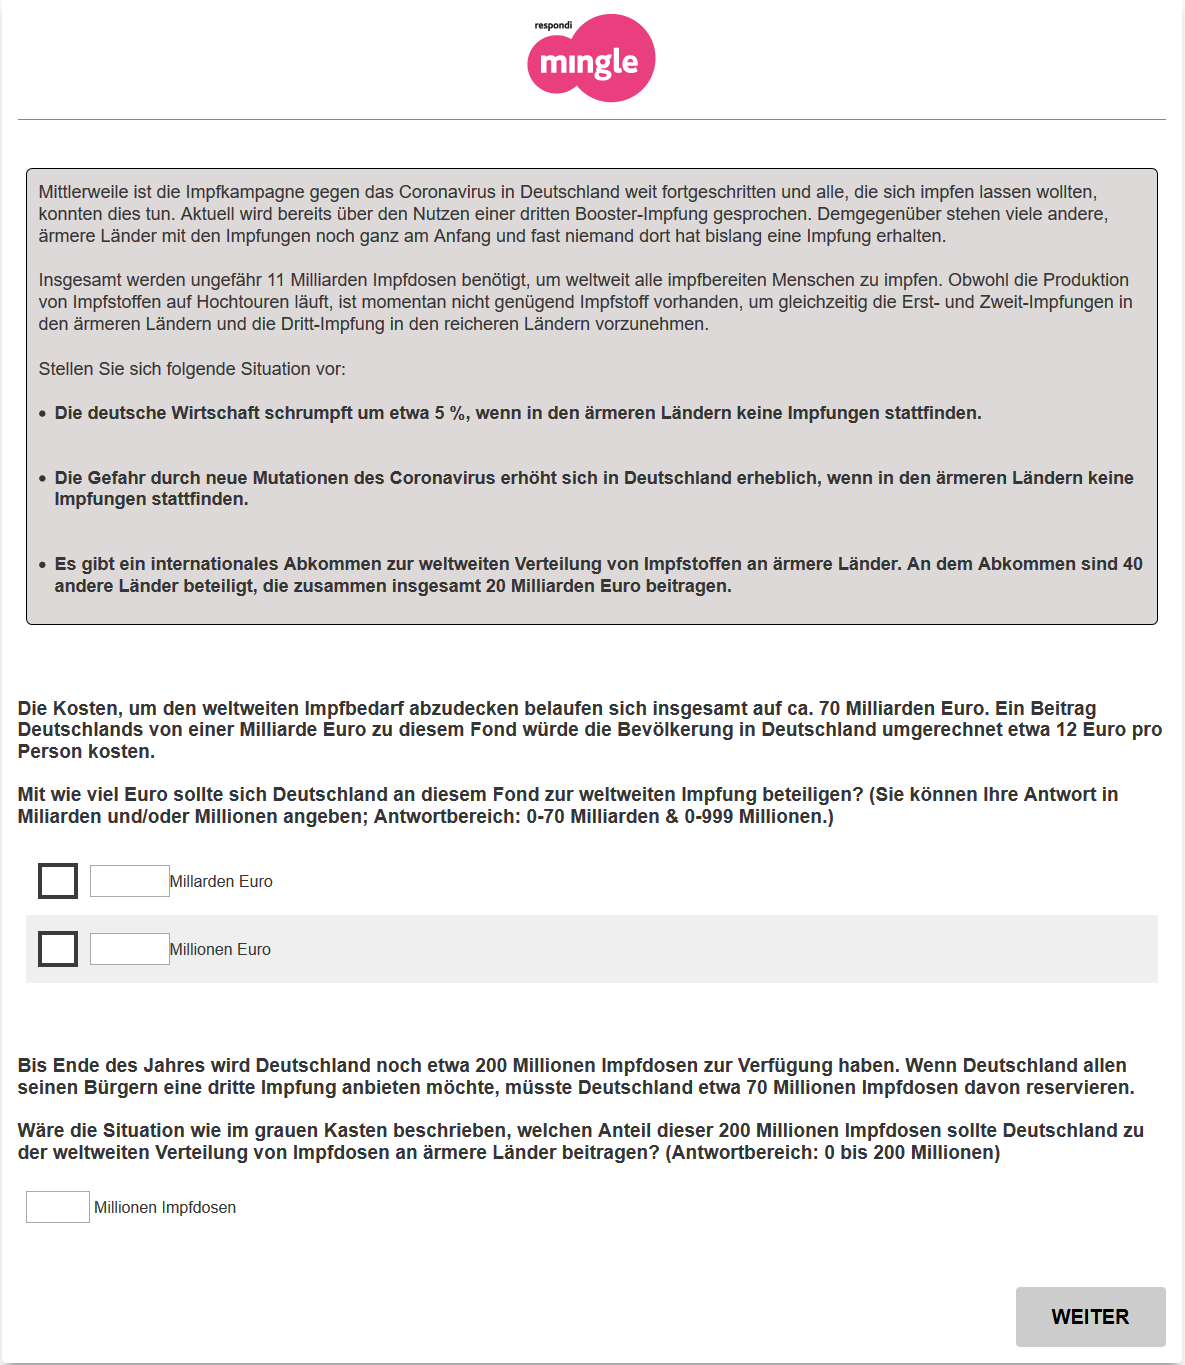
\includegraphics[width=\linewidth]{../Figures/Experiment_8.png}
	\caption{Screenshot of the interface}
	\label{fig:screen}
	%\floatnote{This is a note for this figure.}
\end{figure}




\clearpage
\section{Information Experiment Design}

The information experiment was implemented in Wave 2. The experiment was introduced with the following text:

\begin{itemize}
	\item
	\textbf{Introductory text}: And now we come to the topic of the global
	vaccination campaign. The pandemic can only be defeated if it is
	brought under control globally. In the fight against Covid-19, the
	provision of vaccines is particularly important. The COVAX platform
	was set up under the leadership of the World Health Organization (WHO)
	for the acquisition and fair distribution of vaccines.
\end{itemize}

The treatment, assigned to half of the participants, was a video produced by Deutsche Welle. Deutsche Welle is Germany's foreign broadcaster which is organized under public law and financed by federal tax revenues. The video can be viewed here: 
\url{https://www.dw.com/de/impfstoff-f\%C3\%BCr-entwicklungsl\%C3\%A4nder/av-56554104}

\subsection{Outcome: Willingness to share}

\textbf{Attitudinal outcome}: Would you be willing to personally support the international distribution of vaccines?
\begin{enumerate}
	\item Yes
	\item No 
\end{enumerate}

\hypertarget{outcome-personal-donation}{%
	\subsection{Outcome: Personal
		donation}\label{outcome-personal-donation}}

\begin{itemize}
	\item
	\textbf{Personal donation}: You can also contribute to the global
	distribution of the vaccines yourself. UNICEF is working on behalf of
	the COVAX initiative to ensure that the corona vaccines are made
	available to people in the poorest countries.
	
	Next to the 75 Mingle points that you receive for taking part in this
	survey, you will receive an \textbf{additional 50 Mingle points} from
	us. You can either keep these points yourself or donate all or part of
	them to UNICEF for the worldwide distribution of corona vaccines. For
	every mingle point you donate, we donate 1.5 mingle points to UNICEF.
	
	Please select how the additional Mingle points should be allocated to
	you or UNICEF.
\end{itemize}




\begin{longtable}[]{@{}lll@{}}
	\caption{Bonuses and donations}
	\label{table:mingle}
	\endfirsthead
	\endhead
	\toprule
	& Your Bonus & Donation to UNICEF\tabularnewline
	\midrule
	\endhead
	1 & 0 Mingle Points & 75 Mingle Points\tabularnewline
	2 & 10 Mingle Points & 60 Mingle Punkte\tabularnewline
	3 & 20 Mingle Points & 45 Mingle Points\tabularnewline
	4 & 30 Mingle Points & 30 Mingle Points\tabularnewline
	5 & 40 Mingle Points & 15 Mingle Points\tabularnewline
                                                                            	6 & 50 Mingle Points & 0 Mingle Points\tabularnewline
	\bottomrule
\end{longtable}


\begin{itemize}
	\item
	\emph{Donations go here:}
	https://www.unicef.de/spenden/jetzt-spenden?purpose=235762
\end{itemize}




% \subsection{Wave 2 conjoint}

% In wave 2 of the survey we implemented a Conjoint experiment in which respondents assessed two hypothetical proposals about Germany's contribution to global vaccine sharing. Respondents were asked  to indicate which proposal they would prefer and to rate each proposal with regard to how likely they would vote in favor of or against it in a referendum. The Conjoint experiment allows for estimating the effect of each factor on respondents' preferences for global vaccine sharing. We randomize the following dimensions: contribution to global vaccine sharing, contribution to global vaccine sharing relative to other countries, number of countries participating in global vaccine sharing, economic benefits and health benefits. The factors were assigned with independent probabilities. Each respondent received three vignettes successively. However, respondents did not see that same profile twice. 

% This design differs from the wave 4 design in two important ways. First whereas in wave 4 outcomes included both contributions and doses; the wave 2 design focused on doses only and included the number of doses as part of the conjoint features. Second the economic and health risk items in the wave 2 conjoint implicitly altered the *set* of countries receiving rather than the conditions under which countries receive. In addition the orders of magnitude are not in line with those facing policy makers. 



%\clearpage
%\section{Descriptive Statistics}  

%%%%%%%%%%%%%%%%%

\clearpage
\section{Information experiment results}

Figure \ref{fig:video} reports the results of the information experiment described in Section 3.

\begin{figure}[hbt!]
	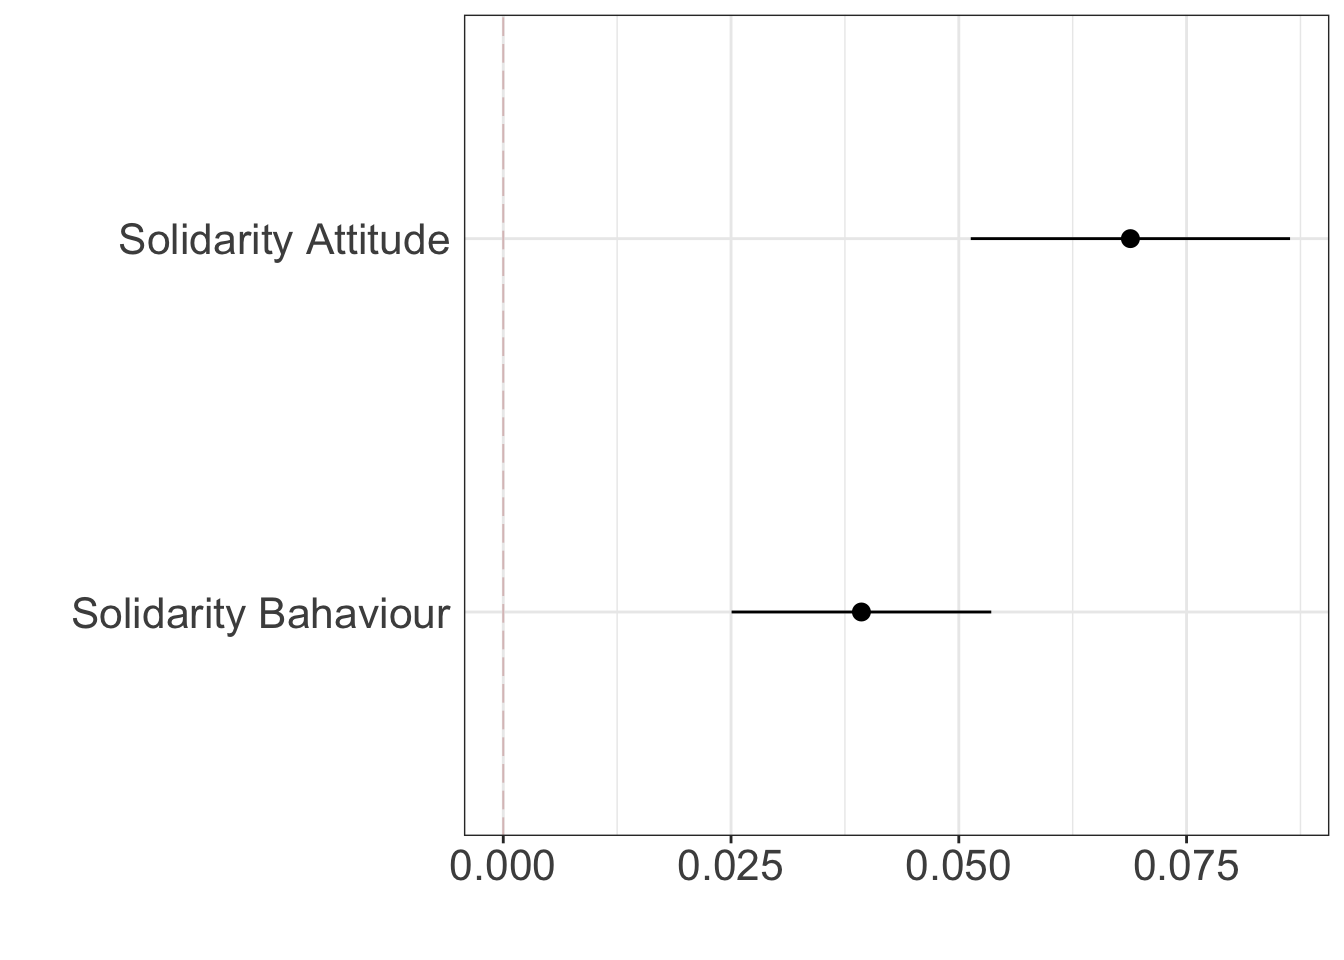
\includegraphics[width=\linewidth]{../Figures/fig_video.png}
	\caption{Effect of video treatment on individual solidarity}
	\label{fig:video}
	%\floatnote{This is a note for this figure.}
\end{figure}

\newpage

\newpage
\section{Pre-registered subgroup analyses}

\begin{figure}[hbt!]
	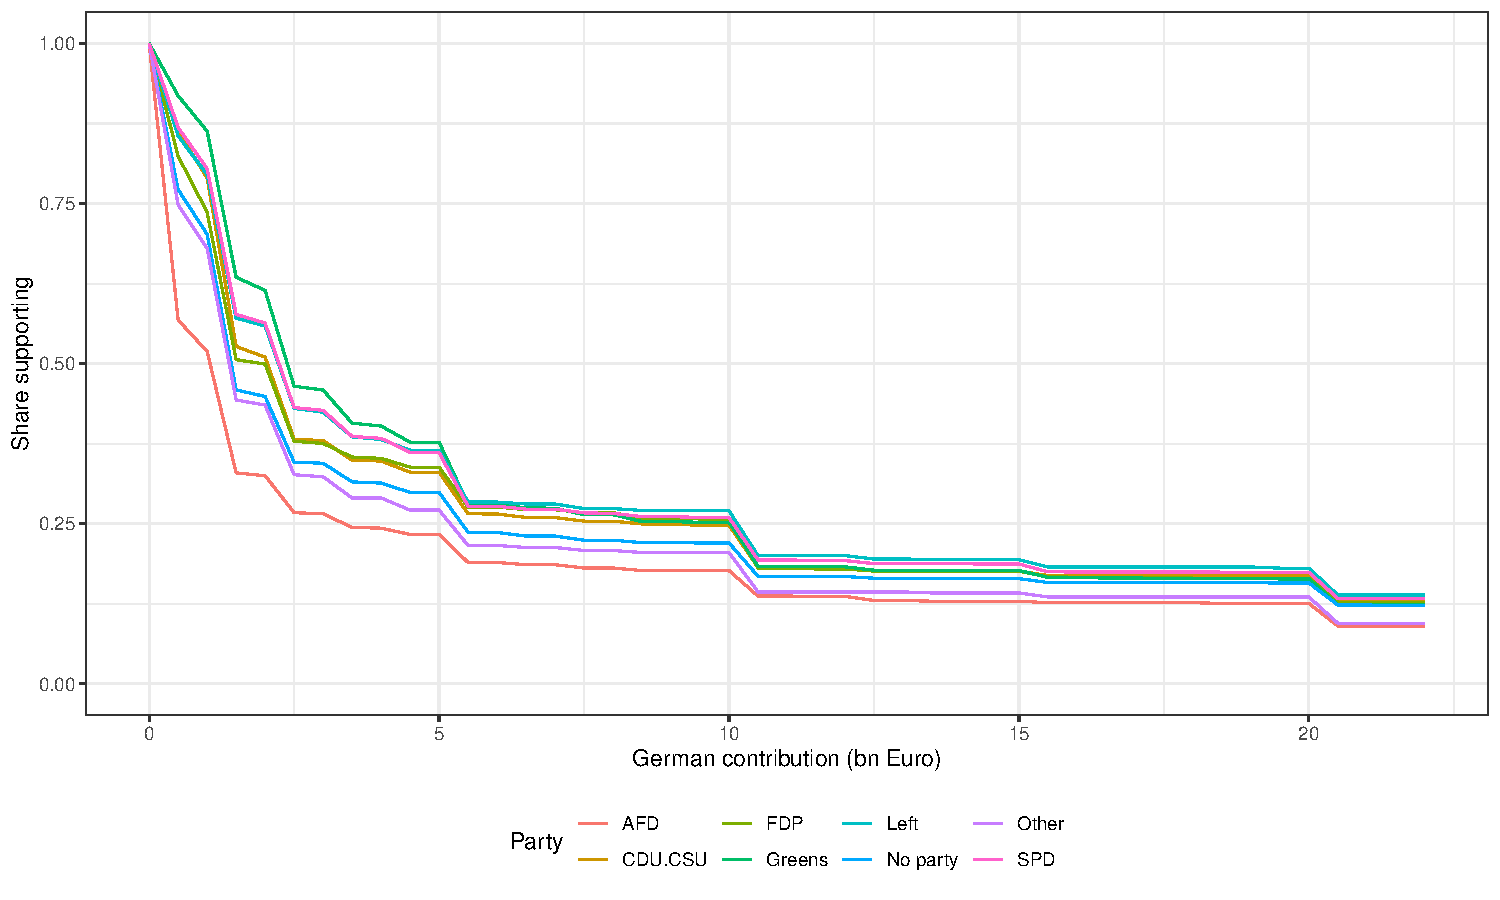
\includegraphics[width=\linewidth]{"../2_output/cumulative_by_party.pdf"}
	\caption{Levels of support by party}
	\label{fig:cuma}
	%\floatnote{This is a note for this figure.}
\end{figure}

\begin{figure}[hbt!]
	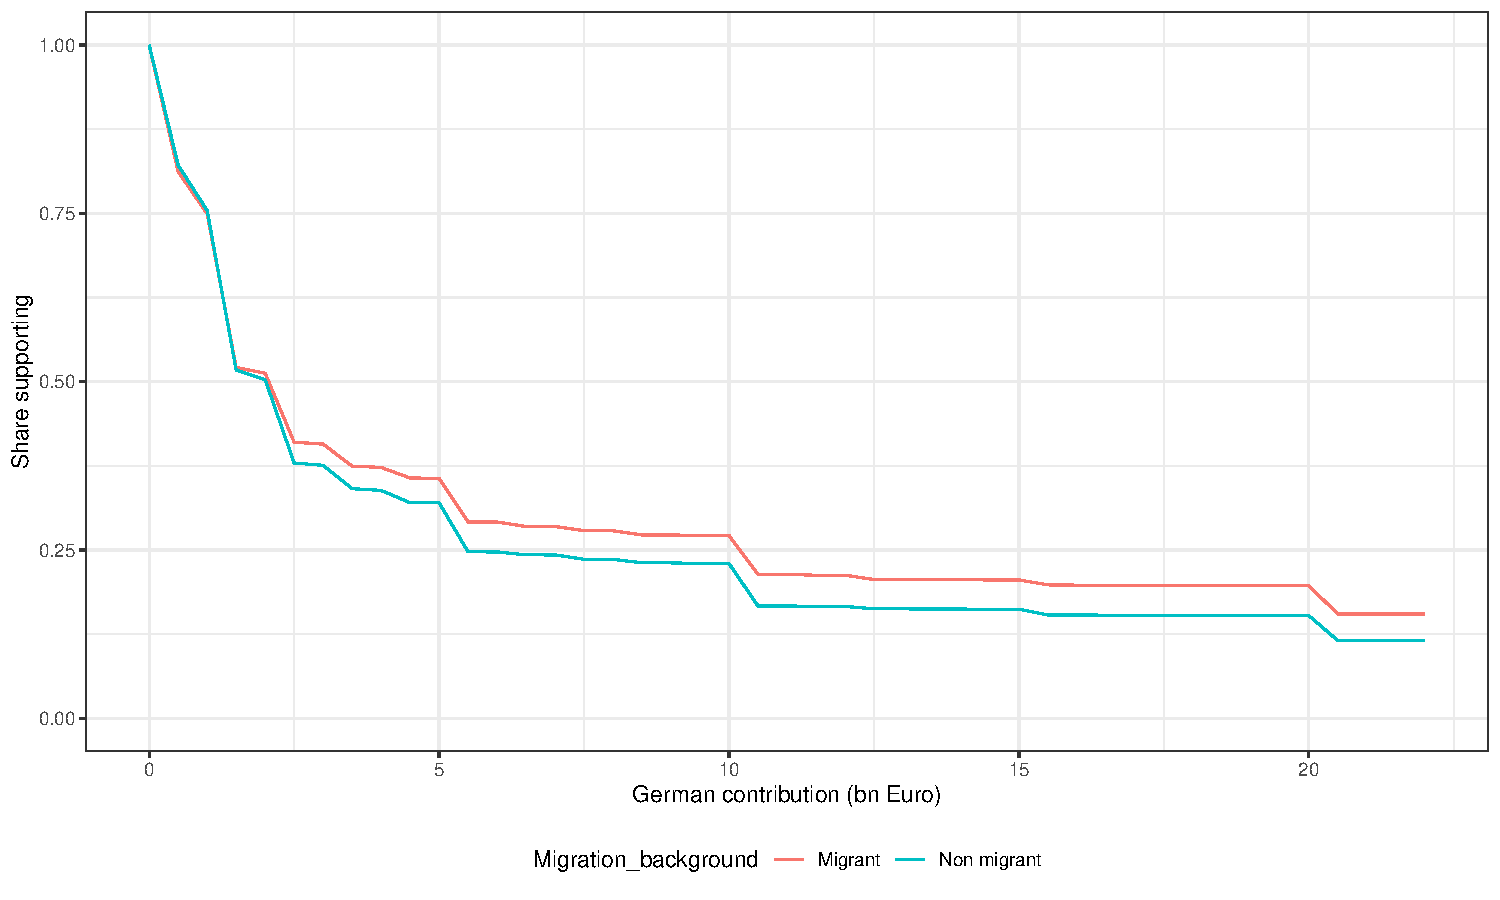
\includegraphics[width=\linewidth]{"../2_output/cumulative_by_migration.pdf"}
	\caption{Levels of support by migration background}
	\label{fig:cumb}
	%\floatnote{This is a note for this figure.}
\end{figure}


\begin{figure}[hbt!]
	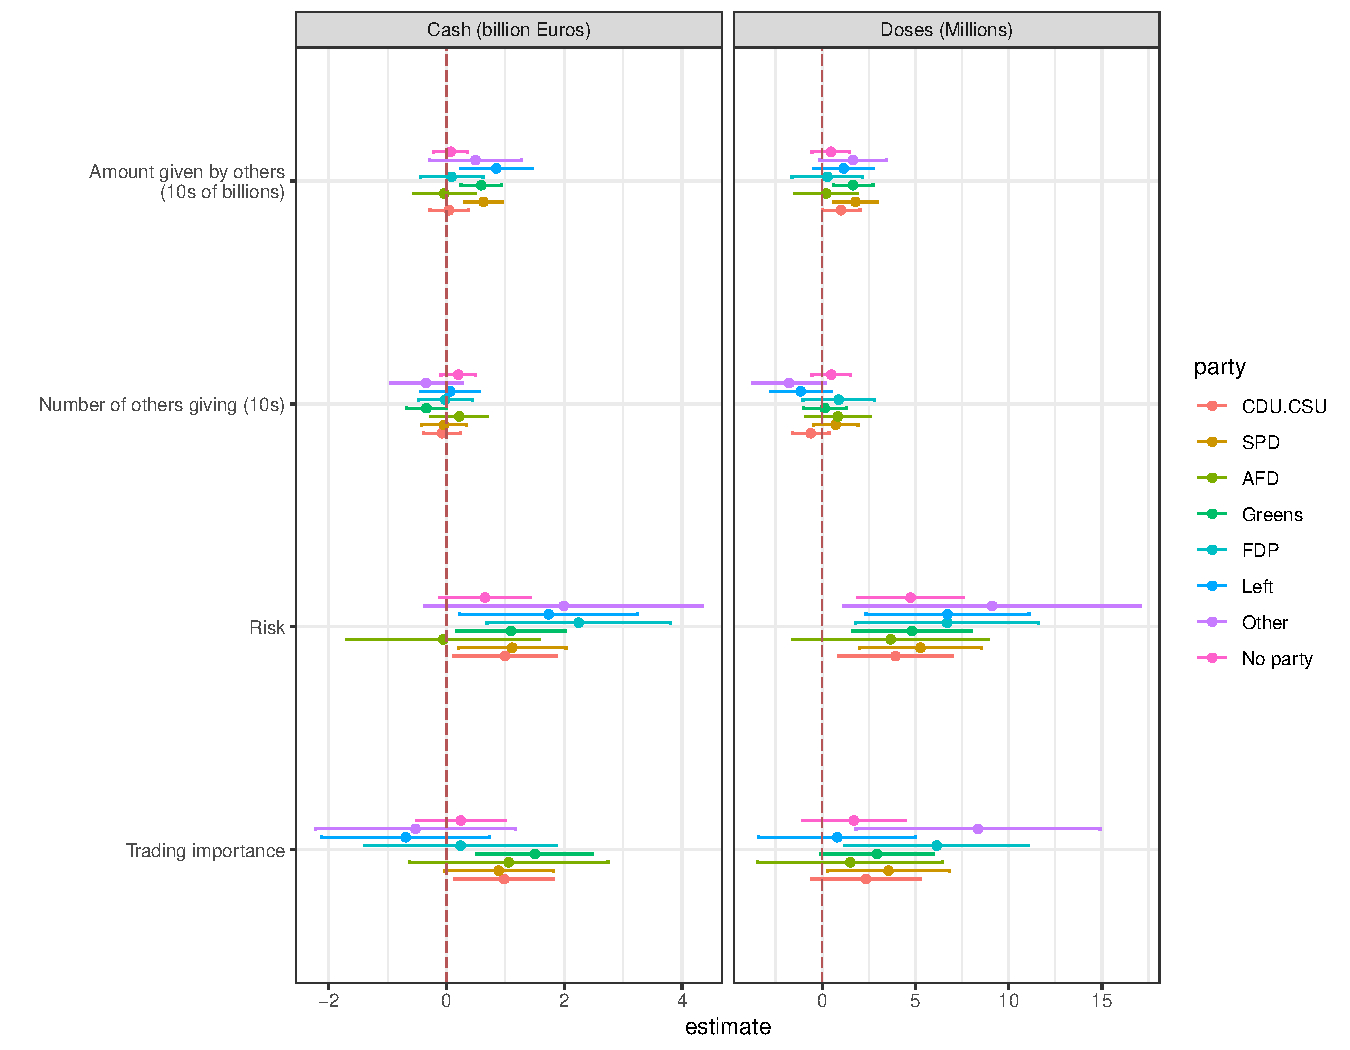
\includegraphics[width=\linewidth]{"../2_output/figure_1_party.pdf"}
	\caption{Marginal effects of conditions by party}
	\label{fig:mainp}
	%\floatnote{This is a note for this figure.}
\end{figure}

\begin{figure}[hbt!]
	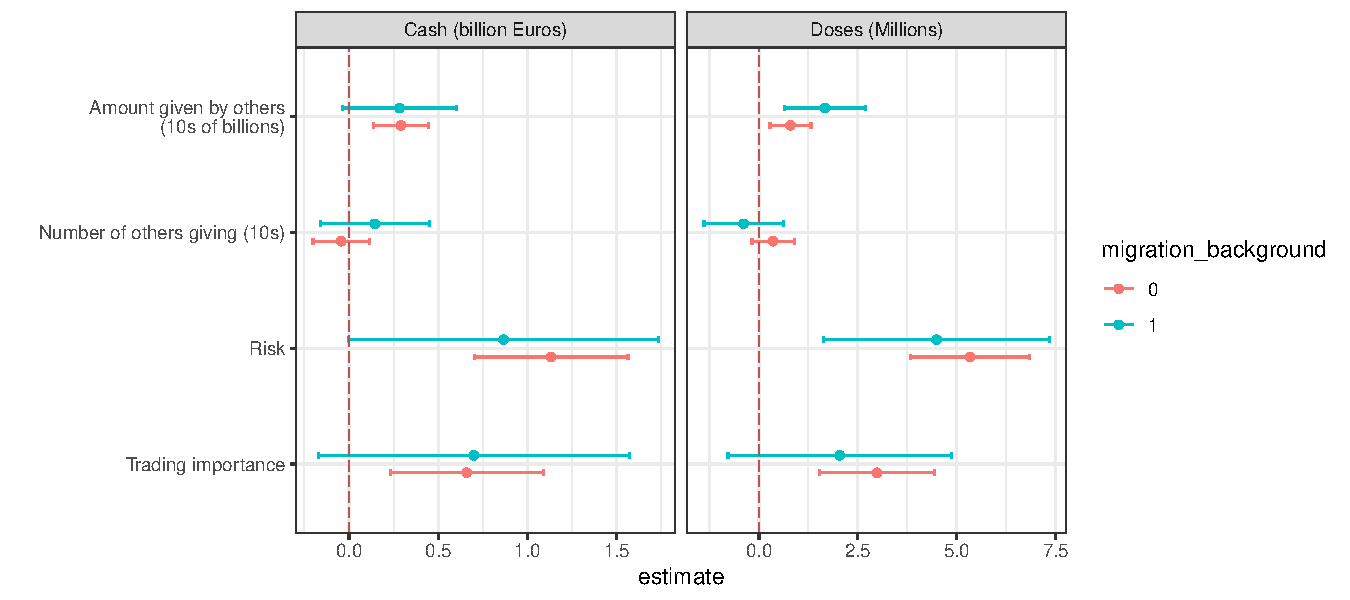
\includegraphics[width=\linewidth]{"../2_output/figure_1_background.pdf"}
	\caption{Marginal effects of conditions by migration background}
	\label{fig:mainb}
	%\floatnote{This is a note for this figure.}
\end{figure}

\end{document}
